\label{anlage:katalog}

Der Anhang dokumentiert den im Berichtszeitraum erreichten Entwicklungsstand der Oberfläche und Navigation des Bauteilkatalogs. Die Screenshots zeigen Zwischenstände und keinen abgeschlossenen Funktionsumfang.

\begin{center}
Bauteilobjekt\\[2mm]
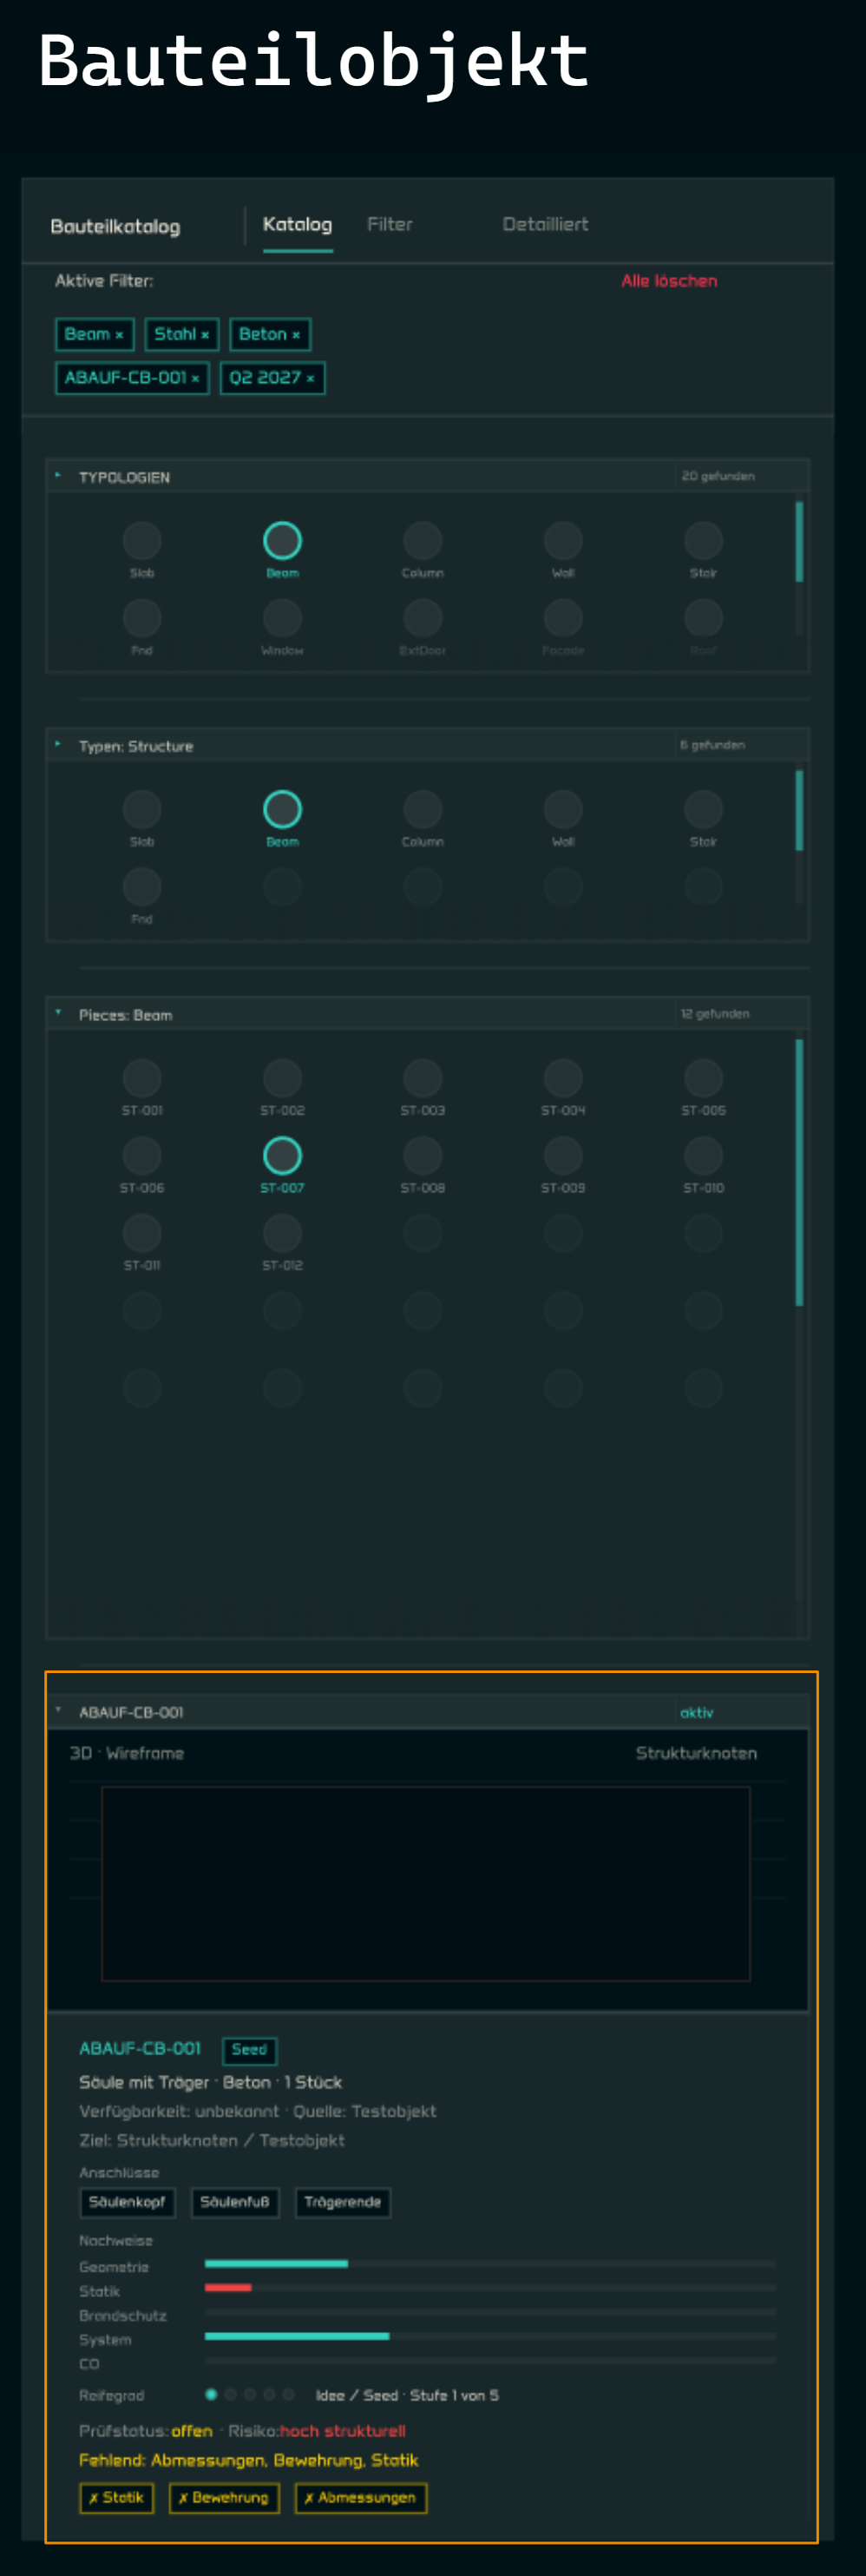
\includegraphics[width=5.5cm]{🖼️asset/📚️katalog/🧱️bauteilobjekt.png}
\end{center}

Die Katalognavigation führt von der Typologienübersicht über die Typen einer Struktur bis zu den einzelnen Bauteilen (Pieces). Das aktive Bauteilobjekt ABAUF-CB-001 zeigt Anschlüsse, den Nachweisstatus je Fachbereich (Geometrie, Statik, Brandschutz, System, CO\textsubscript{2}) sowie den Reifegrad.

\begin{center}
Filteransicht\\[2mm]
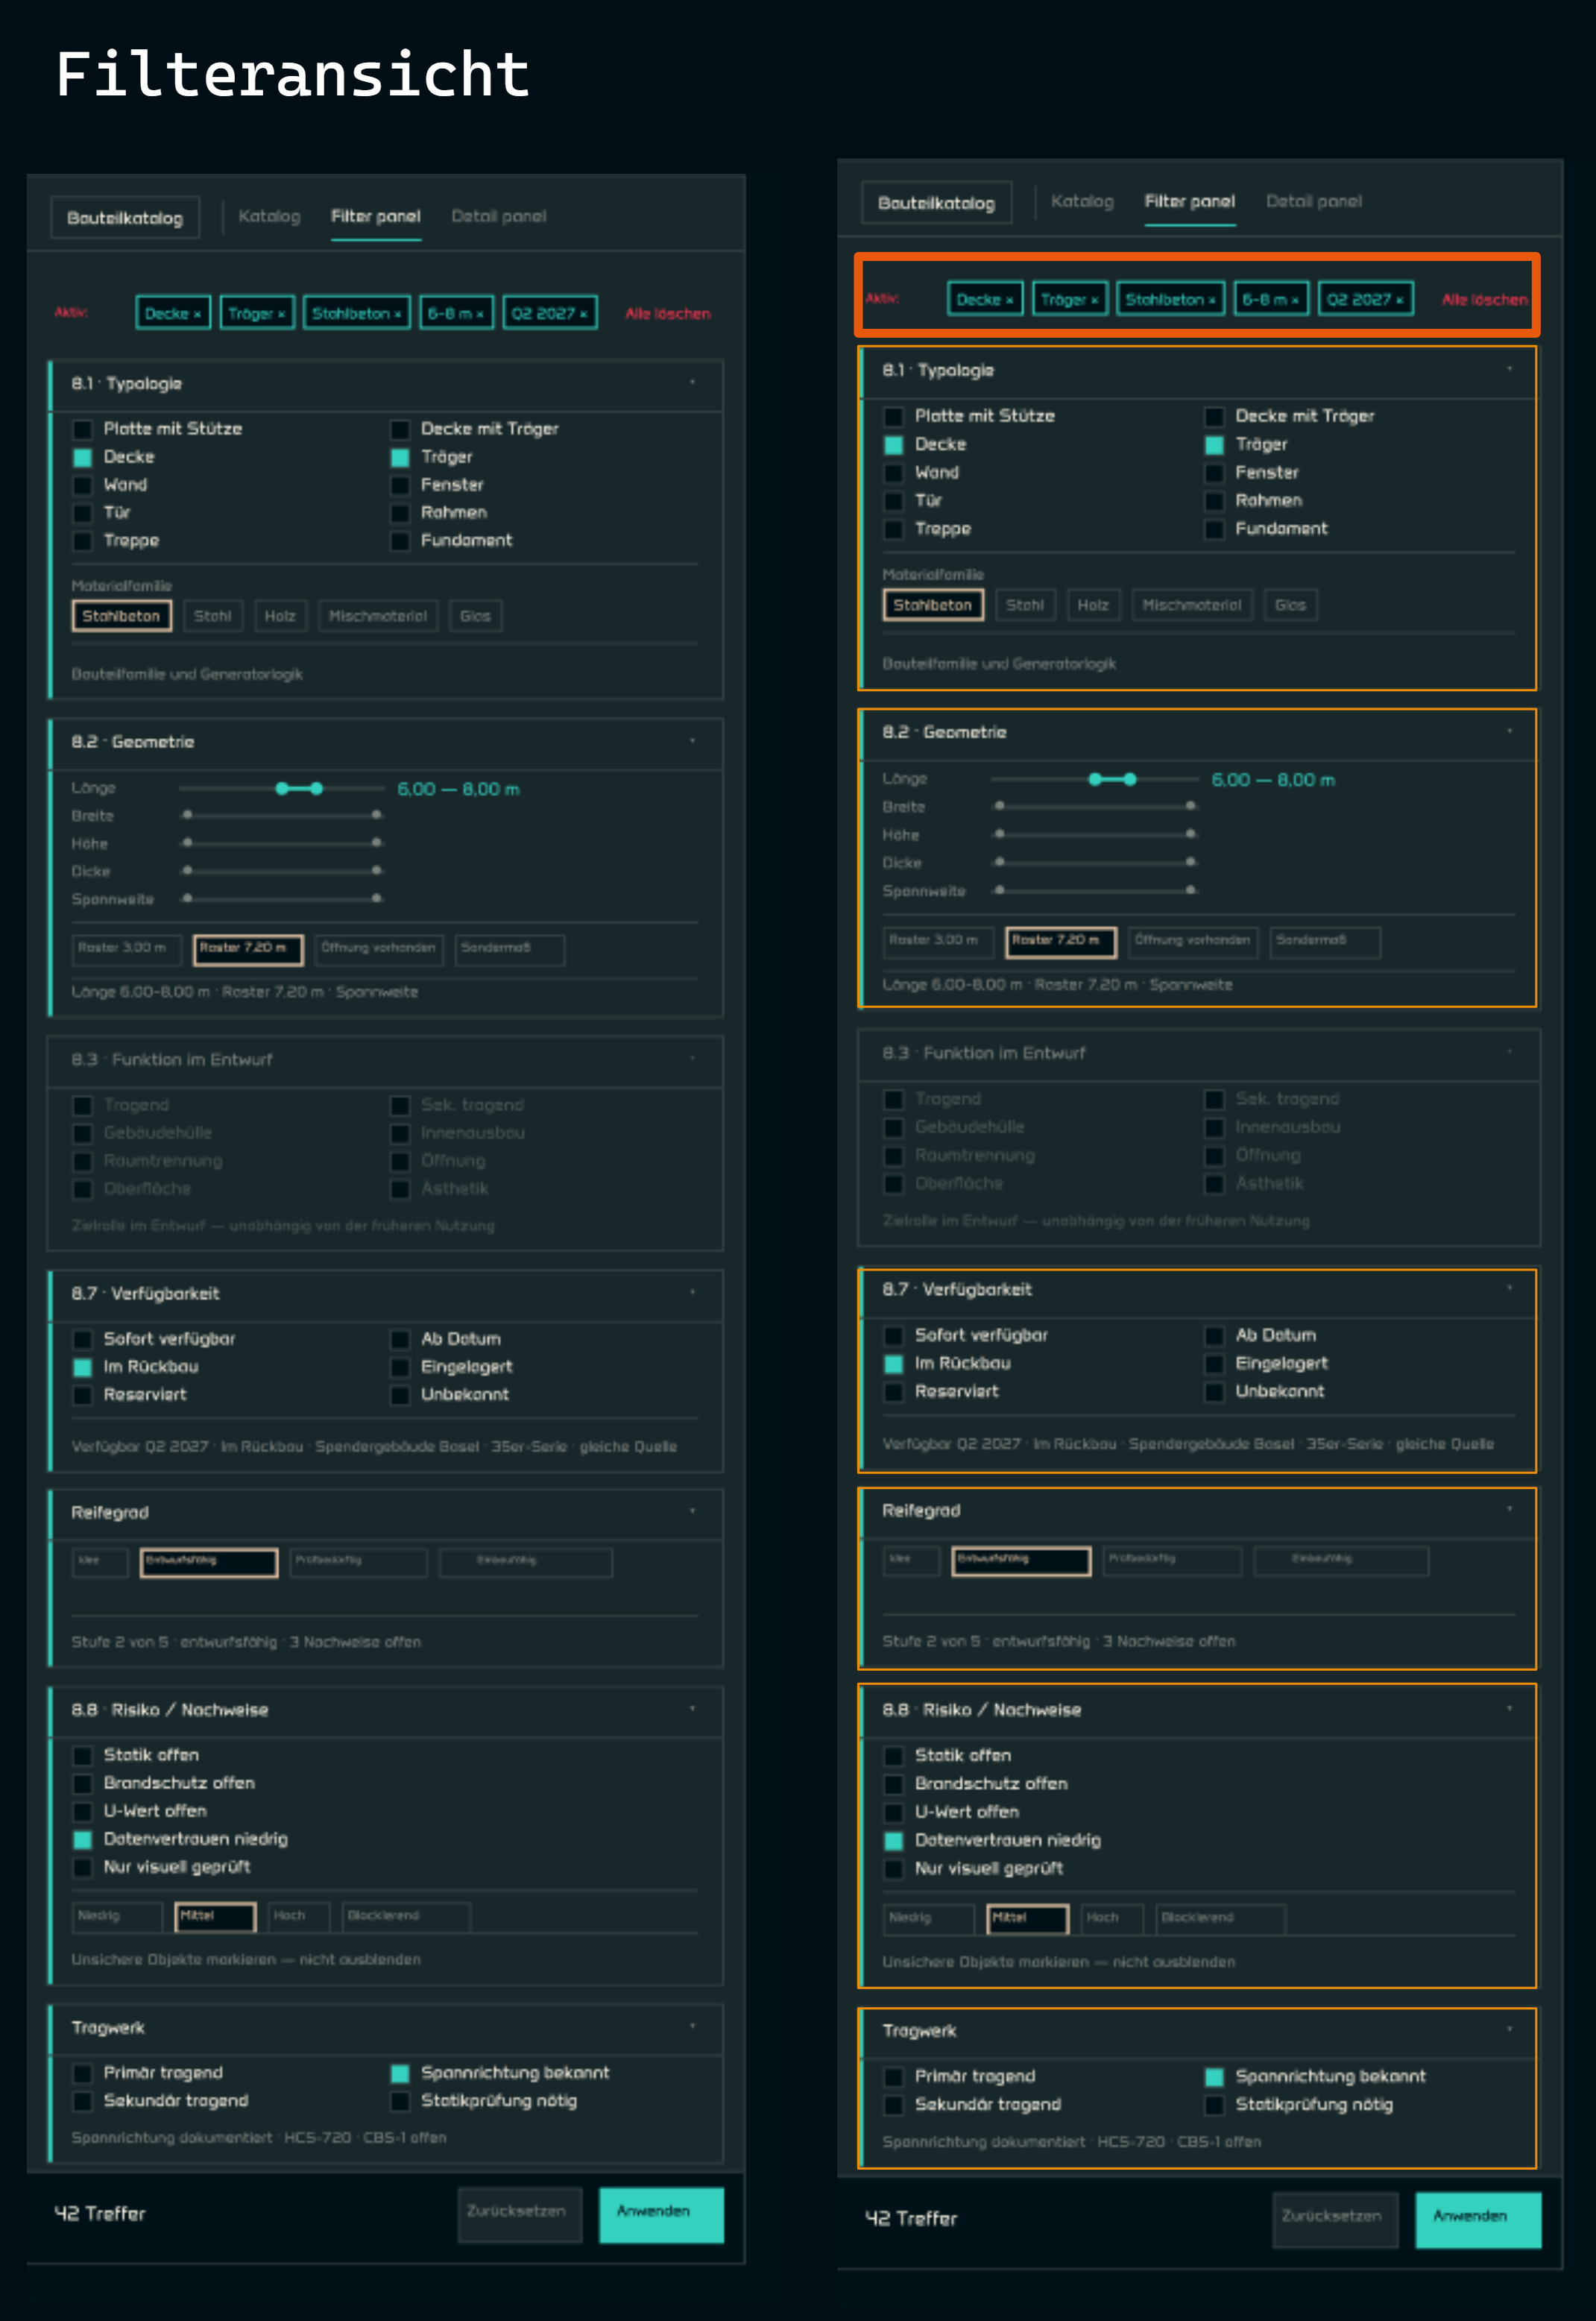
\includegraphics[width=13.5cm]{🖼️asset/📚️katalog/🧮️filteransicht.png}
\end{center}

Das Filter-Panel gliedert Filterkriterien nach Typologie, Materialfamilie, Geometrie, Funktion im Entwurf, Verfügbarkeit, Reifegrad sowie Risiko und Nachweise. Aktive Filter werden als Chips oberhalb der Kriteriengruppen zusammengefasst.

\begin{center}
Bauteilkarte\\[2mm]
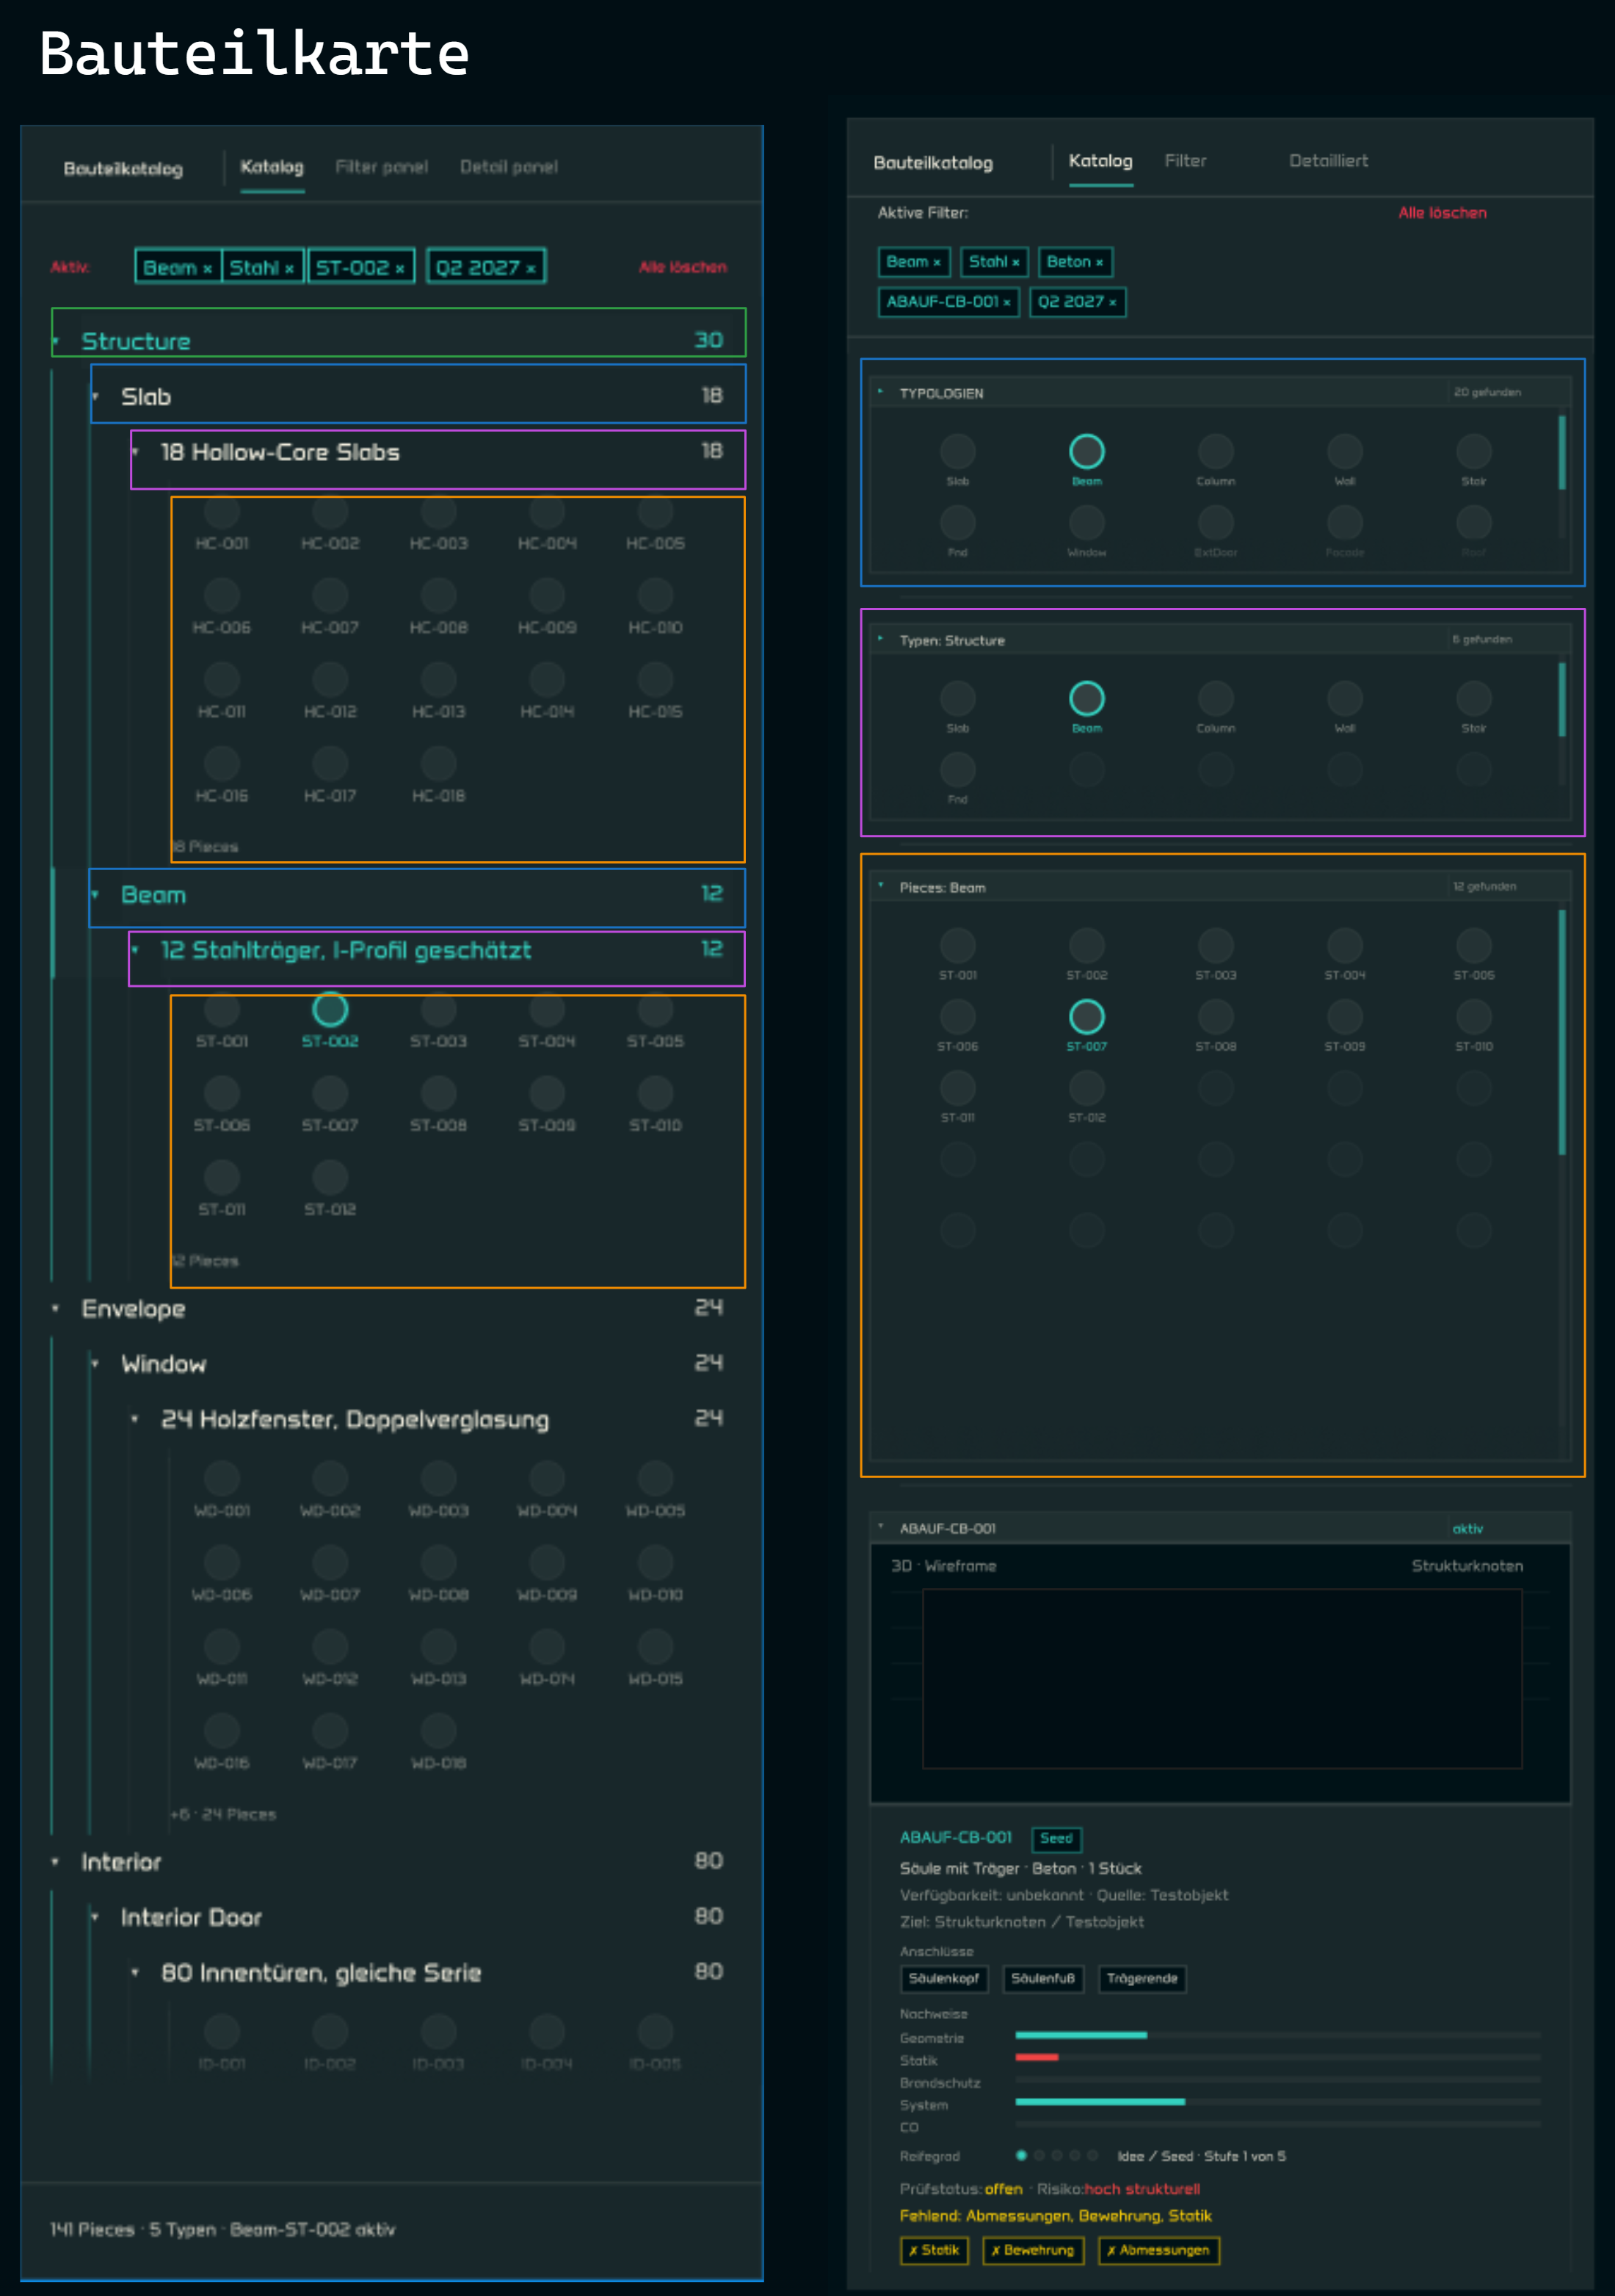
\includegraphics[width=13.5cm]{🖼️asset/📚️katalog/🪪️bauteilkarte.png}
\end{center}

Der hierarchische Katalogbaum gliedert die Bauteile nach Systemebene und Typ. Die Bauteilkarte am unteren Rand bündelt Geometrie, Anschlüsse und Nachweise des ausgewählten Bauteils. Die englischen Ebenenbezeichnungen Structure, Envelope und Interior bleiben als Bezeichnungen der Benutzeroberfläche erhalten und werden beim ersten Auftreten kurz erläutert.
